\chapter{Results and discussions}
\label{chap:results_discussion}  

\begin{center} % Abstract overview
\singlespacing\parbox{12cm}{\textit{
    Write abstract overview of the chapter here. This will help examiner to see overall contents presented in this chapter. It is recommended to write overview after completing the chapter. The overview must be between 100 and 150 words. An abstract overview is optional if you are writing project report.
    }}
\end{center}

\section{RDT mesh interface overlap: discovery and impact assessment}
\label{sec:rdt-mesh-overlap}

The results in this chapter are grouped into two layers. The first layer is the screening matrix of $18$ guide-vane configurations simulated with the original RDT mesh. The second layer is a sub-sample of $7$ configurations rerun with a corrected RDT mesh after a setup error was identified during post-processing. This section documents the error, the discovery, and the validation strategy that ties the two layers together. It is placed first so that every subsequent quantitative claim can be interpreted against the same caveat.

\subsection{Nature of the setup error}
\label{sec:rdt-mesh-overlap-nature}

The rotor domain and the hub-pipe domain of the RDT share a cylindrical interface at $r_\mathrm{hub} = 0.120$~m. The TurboGrid mesh on the rotor blades extends $0.0326$~mm radially beyond this interface and overlaps with the hub-pipe mesh on the hub-blade boundary. CFX resolved this overlap during preprocessing by treating the overlapping nodes as a no-slip wall. The result is an effective interior wall along the hub-blade interface of the RDT, separating the rotor-domain outer flow from the hub-pipe interior flow. The effect is local to the hub region and does not affect the GV passage or the cone-bend section directly.

The consequence is that fluid which should have recirculated through the hub-pipe interior is blocked. Figure~\ref{fig:rdt-mesh-overlap-cc500} shows the original and corrected setup for configuration \texttt{CC\_500\_8}. In the original setup the pressure field shows discontinuous bands at the hub boundary (panel~a), and the velocity vectors stop at the artificial wall instead of crossing it (panel~b). In the corrected setup the pressure field is continuous across the hub boundary (panel~c), and the velocity vectors pass through the hub pipe as expected for a hubless rim-driven thruster (panel~d). The same difference appears in the swirl-only reference simulation (Figure~\ref{fig:rdt-mesh-overlap-swirl}). The downstream pressure level is lower and the radial pressure gradient at the hub is smoother in the corrected case.

\begin{figure}[H]
\centering
\begin{subfigure}[t]{0.48\linewidth}
    \centering
    \includegraphics[width=\linewidth]{Figures/RDT_mesh_error/CC_500_8_wrong_pressure.png}
    \caption{Original (wrong) -- pressure}
\end{subfigure}\hfill
\begin{subfigure}[t]{0.48\linewidth}
    \centering
    \includegraphics[width=\linewidth]{Figures/RDT_mesh_error/CC_500_8_correct_pressure.png}
    \caption{Corrected -- pressure}
\end{subfigure}

\vspace{0.6em}

\begin{subfigure}[t]{0.48\linewidth}
    \centering
    \includegraphics[width=\linewidth]{Figures/RDT_mesh_error/CC_500_8_wrong_velocity.png}
    \caption{Original (wrong) -- velocity}
\end{subfigure}\hfill
\begin{subfigure}[t]{0.48\linewidth}
    \centering
    \includegraphics[width=\linewidth]{Figures/RDT_mesh_error/CC_500_8_correct_velocity.png}
    \caption{Corrected -- velocity}
\end{subfigure}
\caption{Configuration \texttt{CC\_500\_8}: pressure contours (top) and velocity vectors (bottom) on a $zy$-plane cutting through the RDT hub region. The original mesh imposes an artificial no-slip wall along the rotor--hub interface, visible as discontinuous pressure bands and velocity vectors that terminate at the boundary. The corrected mesh removes the $0.0326$~mm radial overlap and restores continuous flow through the hub pipe.}
\label{fig:rdt-mesh-overlap-cc500}
\end{figure}

\begin{figure}[H]
\centering
\begin{subfigure}[t]{0.48\linewidth}
    \centering
    
\includegraphics[width=\linewidth]{Figures/RDT_mesh_error/Swirl_wrong_pressure_contour.png}
    \caption{Original (wrong) RDT setup}
\end{subfigure}\hfill
\begin{subfigure}[t]{0.48\linewidth}
    \centering
    
\includegraphics[width=\linewidth]{Figures/RDT_mesh_error/Swirl_correct_pressure_contour.png}
    \caption{Corrected RDT setup}
\end{subfigure}
\caption{NoGV swirl reference: full-length pressure field on a meridional plane. The corrected setup shows a smoother pressure distribution through the hub region and a different absolute pressure level downstream. The downstream cone--bend topology is identical in both cases.}
\label{fig:rdt-mesh-overlap-swirl}
\end{figure}

\subsection{Why standard sanity checks did not flag the error}
\label{sec:rdt-mesh-overlap-why-missed}

Five routine checks were performed during the screening campaign. None of them flagged the interface overlap. Mass-flow conservation between inlet and outlet was satisfied to better than $0.1\%$ in all $18$ cases, because the displaced fluid was rerouted around the hub wall rather than lost. The $y^+$ distribution on the RDT blade and the draft-tube wall remained inside the intended log-law range, since the artificial wall added new boundary nodes but did not violate the wall-treatment assumption. The frozen-rotor pressure jump at the rotor--stator interface was within the magnitude seen in earlier work in the project and was interpreted as a normal interface transition. RMS residuals converged to below $10^{-5}$. Monitor values stabilised within the prescribed iteration window.

The error was identified during post-processing of velocity vectors on a $zy$-plane through the RDT, when a visible row of stagnant vectors was observed along the hub-blade boundary. The hub-pipe interior also showed an unphysical near-stagnant region. A subsequent inspection of the TurboGrid blade mesh and the hub-pipe mesh confirmed the $0.0326$~mm radial overlap.

\subsection{Corrected sub-sample: seven anchor cases}
\label{sec:rdt-mesh-overlap-validation}

A complete rerun of all $18$ configurations was not feasible within the time available. Seven configurations were selected as anchor points and rerun with the corrected RDT mesh: the NoGV swirl reference, three \texttt{CC} cases (\texttt{CC\_250\_9}, \texttt{CC\_450\_6}, \texttt{CC\_500\_8}), and four \texttt{CS} cases (\texttt{CS\_250\_9}, \texttt{CS\_450\_6}, \texttt{CS\_500\_6}, \texttt{CS\_500\_8}). The selection spans both families, three chord levels, and the corners of the design space relevant to the Pareto analysis presented later in this chapter. Two of the four uncorrected Pareto-front cases, \texttt{CC\_500\_8} and \texttt{CS\_500\_6}, are included as anchors; the remaining two, \texttt{CC\_400\_8} and \texttt{CS\_500\_8}, are partially covered (\texttt{CS\_500\_8} is anchored, \texttt{CC\_400\_8} is not). The implication of the missing \texttt{CC\_400\_8} anchor is discussed in Section~\ref{sec:rdt-mesh-overlap-impact}.

Table~\ref{tab:correctRDT-anchor} lists the original and corrected values of two principal metrics: the system head increase $\Delta H_\mathrm{sys} = H_\mathrm{ConeEnd} - H_\mathrm{RDTStart}$ and the mass-averaged absolute flow angle $|\alpha|$ at \texttt{ConeEnd}. The table guides three observations that shape the rest of the chapter.

The NoGV reference and the GV cases move in opposite directions. The corrected NoGV reference shows higher $\Delta H_\mathrm{sys}$ ($+6.2\%$) and higher $|\alpha|$ ($+18.8\%$) than the original. Without guide vanes, removing the artificial hub wall allows a stronger and more developed swirling flow to leave the RDT, and both throughflow head and residual swirl increase. With guide vanes, $\Delta H_\mathrm{sys}$ drops by $7$ to $14\%$ and $|\alpha|$ drops by $2$ to $32\%$. The cleaner upstream inflow lets the vanes recover more swirl, so the residual angle falls. Some of the recovered momentum is lost as additional vane-passage head loss.

The magnitudes of the changes vary substantially between cases. For $|\alpha|$ the corrected change ranges from $-1.7\%$ (\texttt{CS\_450\_6}) to $-31.5\%$ (\texttt{CC\_500\_8}), almost a factor of $20$. The corresponding spread for $\Delta H_\mathrm{sys}$ is narrower ($-7.0\%$ to $-13.7\%$) but still significant. The bias is therefore case-dependent in magnitude, not a uniform shift that could be cancelled by a single correction factor.

Directional consistency holds for $\Delta H_\mathrm{sys}$ and $|\alpha|$ across the seven GV cases (both quantities decrease after correction) but not for every metric. The head loss in the guide-vane passage ($\mathrm{HL}_\mathrm{GVStart \to z680}$) decreases for five anchor cases (range $-0.4\%$ to $-12.8\%$) but increases for two: \texttt{CS\_450\_6} ($+8.6\%$) and \texttt{CS\_500\_6} ($+15.4\%$). The sign reversal is consistent with how each GV geometry interacts with the upstream wake structure that the artificial hub wall had distorted, but it shows that no single rule for the bias direction applies to every quantity.

\begin{table}[H]
\centering
\small
\caption{Anchor sub-sample: original and corrected values for system head increase $\Delta H_\mathrm{sys}$ and mass-averaged absolute flow angle $|\alpha|$ at \texttt{ConeEnd}. Relative change is $X^\mathrm{corr}/X^\mathrm{orig} - 1$ in percent. Values are read from \texttt{Results\_correctRDT.csv}.}
\label{tab:correctRDT-anchor}
\begin{tabular}{l rrr rrr}
\hline
     & \multicolumn{3}{c}{$\Delta H_\mathrm{sys}$ (m)} & \multicolumn{3}{c}{$|\alpha|$ at ConeEnd (deg)} \\
Case & orig & corr & $\Delta$ (\%) & orig & corr & $\Delta$ (\%) \\ \hline
NoGV swirl          & 3.96 & 4.21 & $+6.2$   & 53.6 & 63.7 & $+18.8$ \\
\texttt{CC\_250\_9} & 3.70 & 3.43 & $-7.5$   & 35.0 & 30.7 & $-12.2$ \\
\texttt{CC\_450\_6} & 3.74 & 3.29 & $-12.0$  & 25.5 & 21.9 & $-14.3$ \\
\texttt{CC\_500\_8} & 3.74 & 3.33 & $-10.9$  & 16.5 & 11.3 & $-31.5$ \\
\texttt{CS\_250\_9} & 3.62 & 3.12 & $-13.7$  & 35.1 & 33.5 & $-4.6$  \\
\texttt{CS\_450\_6} & 3.49 & 3.19 & $-8.7$   & 22.3 & 22.0 & $-1.7$  \\
\texttt{CS\_500\_6} & 3.32 & 3.09 & $-7.0$   & 13.1 & 12.3 & $-6.3$  \\
\texttt{CS\_500\_8} & 3.23 & 2.91 & $-10.1$  &  9.1 &  7.9 & $-13.0$ \\ \hline
\end{tabular}
\end{table}

\subsection{What is preserved, what is biased, and how to read the rest of this chapter}
\label{sec:rdt-mesh-overlap-impact}

The sub-sample is too small to validate every individual ranking in the $18$-case matrix. It is large enough to identify which classes of claim survive the correction and which classes do not.

Three classes of claim survive the correction. Family-level trends (\texttt{CC} versus \texttt{CS}) are preserved in every comparison performed on the anchor data. The \texttt{CC} family has lower vane-passage head loss than \texttt{CS} in both setups, and the \texttt{CS} family has lower residual flow angle than \texttt{CC} in both setups. Within-family chord trends are also preserved. Longer chord gives lower residual angle in both \texttt{CC} and \texttt{CS} families, in both setups. The direction of the head-loss versus swirl-recovery trade-off is the same in both setups: configurations with stronger swirl recovery pay a higher head-loss penalty.

One class of claim does not survive without qualification. Individual rankings between two cases of the same family and similar chord can change between the two setups. The non-uniform bias in vane-passage head loss documented in Section~\ref{sec:rdt-mesh-overlap-validation} is the direct cause. Where an individual ranking matters for a design recommendation, the value from the corrected anchor is preferred when available, and the limitation is stated explicitly.

The Pareto-front membership is partially confirmed. Four cases are Pareto-dominant in the uncorrected $18$-case matrix: \texttt{CS\_500\_8}, \texttt{CS\_500\_6}, \texttt{CC\_500\_8} and \texttt{CC\_400\_8}. Three of these are present in the corrected anchor set (\texttt{CS\_500\_8}, \texttt{CS\_500\_6}, \texttt{CC\_500\_8}) and remain Pareto-dominant within that sub-sample. \texttt{CC\_400\_8} was not rerun and its Pareto status cannot be verified. A fourth case, \texttt{CC\_250\_9}, appears on the Pareto front of the corrected sub-sample because it is the highest-$\Delta H_\mathrm{sys}$ case among the seven anchors. This is a sub-sample artefact rather than evidence of a new Pareto-dominant design, since the larger uncorrected matrix shows several \texttt{CC} cases with higher $\Delta H_\mathrm{sys}$ and lower $|\alpha|$ than \texttt{CC\_250\_9}. The final candidate selection in the synthesis section of this chapter therefore relies on the three anchor-confirmed Pareto candidates and treats \texttt{CC\_400\_8} as an unverified candidate.

Four reading rules follow from this analysis. They apply to every quantitative claim in the remainder of the chapter.

\begin{enumerate}
    \item Family-level trends (\texttt{CC} vs \texttt{CS}) and within-family chord trends are stated as primary findings.
    \item Individual rankings between two cases of the same family and similar chord are stated only where they are robust across both setups, or where the anchor value confirms them. When they are not robust, the limitation is named.
    \item Absolute values of $\Delta H_\mathrm{sys}$, head-loss components and pressure recovery are reported as comparison values, not as design predictions. The bias on $\Delta H_\mathrm{sys}$ is $-7$ to $-14\%$ for the GV cases in Table~\ref{tab:correctRDT-anchor}.
    \item Cavitation margins, axial forces and runner torque carry independent uncertainty -- the CFX reference pressure used for cavitation evaluation was not set with the precision required for quantitative cavitation prediction -- and are used as qualitative diagnostics only.
\end{enumerate}

Results from the seven corrected anchor cases are reported alongside the uncorrected screening results where the comparison is informative. The screening matrix remains the $18$ uncorrected cases. Re-running all $18$ configurations with the corrected RDT mesh is identified as the principal item of future work and is discussed in Chapter~\ref{chap:future_work}.

\section{Reference behaviour and validation}
\label{sec:reference-and-validation}

The screening matrix produces eighteen numbers per metric. Before interpreting them, two reference simulations anchor the meaning of those numbers. The NoGV swirl reference (RDT operating without guide vanes) sets the upper bound on residual swirl and on bend head loss, and defines the baseline that every guide-vane configuration is designed to improve. The NoGV straight validation (no RDT, axial inlet) tests whether the cone-bend domain itself introduces artificial swirl that could contaminate the comparison. Mass conservation and the wall-treatment strategy are then documented for the full $18$-case matrix.

\subsection{NoGV swirl reference}
\label{sec:nogv-swirl-reference}

The NoGV swirl reference simulates the corrected RDT with the same downstream domain (cone, $90^\circ$ bend, final pipe) but without any guide vanes in place. The flow leaves the RDT, expands into the cone, passes through the bend, and exits at \texttt{ConeEnd}. Without a swirl-recovery element, the tangential momentum imparted by the rotor is carried all the way through the duct.

Table~\ref{tab:nogv-swirl-reference} lists the principal metrics in both the original and corrected setup. The mean flow angle at \texttt{ConeEnd} reaches $63.7^\circ$ in the corrected setup, with an absolute swirl number of $5.35$. The best guide-vane configuration in the screening matrix (\texttt{CS\_500\_8}) reduces $|\alpha|_{\mathrm{ConeEnd}}$ to $9.1^\circ$ uncorrected and to $7.9^\circ$ corrected. The screening matrix therefore covers roughly an eight-fold reduction in residual angle and a twenty-fold reduction in swirl-number magnitude relative to the no-GV reference. Configurations near the worst end of the matrix (\texttt{CS\_250\_9}, \texttt{CC\_250\_9}) still leave $|\alpha|_{\mathrm{ConeEnd}}$ above $30^\circ$; configurations near the best end approach $10^\circ$.

\begin{table}[H]
\centering
\small
\caption{NoGV swirl reference: principal metrics in the original and corrected RDT setup. Mean flow angle and swirl number are taken on the listed planes. $\Delta H_{\mathrm{sys}}$ is $H_{\mathrm{ConeEnd}} - H_{\mathrm{RDTStart}}$. $\mathrm{HL_{Bend}}$ is the head loss between \texttt{BendStart} and \texttt{BendEnd}.}
\label{tab:nogv-swirl-reference}
\begin{tabular}{l rr}
\hline
Metric & Uncorrected & Corrected \\ \hline
$|\alpha|$ at \texttt{ConeEnd} (deg) & $53.6$ & $63.7$ \\
$|S|$ at \texttt{ConeEnd} (-)        & $0.92$ & $5.35$ \\
$|S|$ at \texttt{BendStart} (-)      & $1.52$ & $1.76$ \\
$|S|$ at \texttt{BendEnd} (-)        & $6.62$ & $7.08$ \\
$\Delta H_{\mathrm{sys}}$ (m)        & $3.96$ & $4.21$ \\
$\mathrm{HL_{Bend}}$ (m)              & $0.39$ & $0.37$ \\
\hline
\end{tabular}
\end{table}

The head loss in the bend section is $0.37$~m in the corrected NoGV reference and $0.39$~m in the original. With any guide vane in place, $\mathrm{HL_{Bend}}$ drops to the range $0.014$ to $0.058$~m, an order-of-magnitude reduction. The mechanism behind this collapse is examined in Section~\ref{sec:bend-hl-collapse}. The relevant point in this section is that the bend acts very differently on a strongly swirling flow than on a near-axial flow, and the magnitude of the reduction sets the scale for the head-loss budget across the screening matrix.

The NoGV $|S|$ values increase substantially after the mesh correction. The factor-of-six increase in $|S|$ at \texttt{ConeEnd} ($0.92 \to 5.35$) shows that the artificial hub wall in the original RDT mesh acted as an unintended friction dissipator for tangential momentum. The uncorrected NoGV reference was therefore weaker than the physically correct case. Guide-vane configurations in the uncorrected screening were rated against this weaker reference. The implication is that the guide vanes perform a larger swirl-recovery task than the uncorrected NoGV reference suggests, and that the relative ranking of GV configurations is the appropriate use of the screening data rather than the absolute residual values.

\subsection{NoGV straight validation}
\label{sec:nogv-straight-validation}

The straight-flow validation replaces the RDT with a uniform axial inlet at the bulk velocity $U_b = 2.32$~m/s. There is no rotor, no swirl source, and no rotor-stator interface. The cone-bend domain is otherwise identical to the screening cases. The simulation tests one specific question: does the cone-bend domain introduce in-plane velocity that could contaminate the swirl metrics used in the screening?

The mean flow angle at \texttt{ConeEnd} is $6.8^\circ$. This is not zero, and the residual deserves explanation.

A $90^\circ$ bend induces a counter-rotating Dean-vortex pair through the imbalance between the radial pressure gradient and centrifugal acceleration. The Dean vortices generate in-plane velocity that, when projected onto the cone-axis-normal sampling plane at \texttt{ConeEnd}, registers as a non-zero mean flow angle. The peak normalised in-plane velocity at \texttt{ConeEnd} is $|V_{\mathrm{in\text{-}plane}}|/U_b = 0.51$, and the vector field shows the symmetric counter-rotating pair characteristic of pure bend-induced secondary flow without any external swirl source. The full visualisation is in Figure~\ref{fig:dean-vortex} of Section~\ref{sec:dean-vortex}. The residual is a real bend artefact, not a setup error.

The magnitude of the artefact is small compared to the RDT-induced swirl. The area-averaged swirling strength at \texttt{ConeEnd} is $2.40$~s$^{-1}$ in the straight validation against $25.1$~s$^{-1}$ in the NoGV swirl reference. The validation passes: the cone-bend domain does not produce swirl of the same order as the upstream rotor.

The practical implication is that the $6.8^\circ$ residual sets a floor on what the screening can resolve at \texttt{ConeEnd}. Configurations reporting $|\alpha|_{\mathrm{ConeEnd}}$ in the single-digit range are approaching this floor rather than the ideal axial flow. In the screening matrix, only \texttt{CS\_500\_8} (uncorrected $9.1^\circ$, corrected $7.9^\circ$) falls into this region. Differences between configurations in this range should not be over-interpreted as physical superiority. Section~\ref{sec:swirl-recovery} treats the angle scale near and below $10^\circ$ accordingly.

\subsection{Mass conservation and wall-treatment sanity}
\label{sec:mass-and-yplus}

Two routine checks are required before reporting screening results: mass conservation between domain inlet and outlet, and consistency of the wall treatment strategy across the eighteen cases. Both are documented in Table~\ref{tab:mass-and-yplus}.

Mass conservation is satisfied to better than $0.5\%$ for every case in the screening matrix. The largest negative imbalance is $-0.229\%$ (\texttt{CS\_500\_8}); the largest positive imbalance is $+0.177\%$ (\texttt{CS\_500\_6}). The NoGV swirl reference shows $-0.063\%$. These values are well inside the $1\%$ tolerance used in earlier project work~\cite{Dokset2025, Leonsen2025} and confirm that the steady-state solutions are mass-conservative at the level needed for relative comparison between configurations.

The wall-treatment strategy follows a deliberate compromise. The simulation has three wall types: the guide-vane walls (GV), the RDT blade and hub walls (RDT), and the cone-bend draft-tube walls (DT). The mesh resolution near each wall was chosen with the wall function approach in mind, rather than direct resolution of the viscous sublayer. The SST $k$-$\omega$ turbulence model in CFX uses automatic near-wall treatment, which blends between low-Reynolds integration to the wall (valid for $y^+ < 5$) and wall functions (valid for $30 < y^+ < 300$). Mesh sizing in the present screening was tuned for the wall function regime to keep the total cell count tractable for an $18$-case campaign.

The $y^+$ distribution reflects this choice. GV walls show area-averaged $y^+$ in the range $5$ to $39$ across the screening matrix, straddling the lower transition of the automatic wall treatment. RDT walls (uncorrected setup) show area-averaged $y^+$ in the narrow range $14$ to $16$, comfortably inside the low end of the log-law region. DT walls show the highest values: area-averaged $y^+$ in the range $162$ to $216$, and maximum local $y^+$ between $487$ and $745$.

The DT values are deliberately high. Resolving the DT log-law region with a target maximum $y^+ \lesssim 100$ would have required mesh refinement that increases the cell count by roughly an order of magnitude. The screening matrix would not have been computationally tractable on the available hardware within the project time frame. The screening question is the relative ranking of eighteen GV designs under identical numerical treatment, not the absolute prediction of DT wall friction. The wall function approach handles $y^+$ up to several hundred in CFX automatic mode, and the same mesh strategy is applied to every case, so any DT wall friction bias is consistent across the screening matrix and does not affect relative ranking.

The same logic applies to GV $y^+$. The GV wall mesh is consistent across all eighteen configurations: same boundary-layer extrusion, same first-cell height target, same growth ratio. The differences in $y^+$ between cases reflect differences in local velocity caused by the geometry, not differences in mesh quality. Where individual cases show GV $y^+$ values in the buffer region ($5 < y^+ < 30$) the automatic wall treatment blends both branches, which is its design purpose.

\begin{table}[H]
\centering
\footnotesize
\caption{Mass conservation and $y^+$ distribution for the $18$-case screening matrix and the NoGV swirl reference. $\varepsilon_{\dot m}$ is the inlet-to-outlet mass imbalance in percent. $y^+$ columns are area-averaged values; maximum local values are reported in parentheses for the GV and DT walls. The NoGV reference has no GV walls and the corresponding column is left blank.}
\label{tab:mass-and-yplus}
\begin{tabular}{l r rr r r}
\hline
Case & $\varepsilon_{\dot m}$ (\%) & GV $y^+$ avg (max) & RDT $y^+$ avg & DT $y^+$ avg (max) \\ \hline
\texttt{CS\_500\_8} & $-0.229$ & $5.6$ ($22.9$)  & $15.7$ & $166$ ($745$) \\
\texttt{CS\_500\_6} & $+0.177$ & $5.9$ ($24.1$)  & $15.9$ & $166$ ($699$) \\
\texttt{CS\_450\_8} & $+0.157$ & $18.6$ ($73.1$) & $16.1$ & $175$ ($686$) \\
\texttt{CS\_450\_6} & $+0.025$ & $16.0$ ($53.4$) & $16.1$ & $187$ ($657$) \\
\texttt{CS\_400\_8} & $-0.064$ & $19.8$ ($59.5$) & $16.3$ & $186$ ($589$) \\
\texttt{CS\_400\_6} & $+0.077$ & $18.7$ ($57.9$) & $16.2$ & $194$ ($573$) \\
\texttt{CS\_350\_8} & $+0.152$ & $21.5$ ($57.3$) & $16.3$ & $192$ ($572$) \\
\texttt{CS\_300\_9} & $-0.017$ & $19.6$ ($54.3$) & $16.4$ & $202$ ($488$) \\
\texttt{CS\_250\_9} & $+0.032$ & $14.9$ ($41.9$) & $16.4$ & $216$ ($533$) \\
\texttt{CC\_500\_8} & $+0.025$ & $9.9$  ($30.5$) & $16.4$ & $162$ ($620$) \\
\texttt{CC\_500\_6} & $+0.002$ & $5.8$  ($17.6$) & $16.5$ & $166$ ($520$) \\
\texttt{CC\_450\_8} & $+0.022$ & $22.0$ ($68.5$) & $16.5$ & $172$ ($517$) \\
\texttt{CC\_450\_6} & $-0.004$ & $23.7$ ($73.6$) & $16.4$ & $184$ ($519$) \\
\texttt{CC\_400\_8} & $-0.049$ & $18.6$ ($57.8$) & $16.5$ & $178$ ($504$) \\
\texttt{CC\_400\_6} & $+0.006$ & $18.5$ ($53.7$) & $16.4$ & $198$ ($575$) \\
\texttt{CC\_350\_8} & $-0.035$ & $39.1$ ($116.8$) & $16.5$ & $183$ ($510$) \\
\texttt{CC\_300\_9} & $-0.056$ & $35.2$ ($108.0$) & $16.4$ & $193$ ($544$) \\
\texttt{CC\_250\_9} & $-0.036$ & $34.7$ ($110.6$) & $16.5$ & $209$ ($499$) \\
NoGV swirl          & $-0.063$ & --              & $14.1$ & $396$ ($588$) \\
\hline
\end{tabular}
\end{table}

\section{Head increase and head-loss decomposition}
\label{sec:head-increase-and-hl}

The screening question on the pressure side is straightforward: how much head does each guide-vane configuration deliver to the downstream pump-turbine, and where in the duct is the head loss generated? The first quantity is the system head increase, $\Delta H_{\mathrm{sys}} = H_{\mathrm{ConeEnd}} - H_{\mathrm{RDTStart}}$. The second is the decomposition of the total head loss into three sub-sections: the guide-vane passage, the conical contraction, and the $90^\circ$ bend. Together they identify both the magnitude of the trade-off between configurations and the part of the duct where each configuration pays its penalty.

\subsection{System head increase across the screening matrix}
\label{sec:hi-across-matrix}

Figure~\ref{fig:hi-bar} shows $\Delta H_{\mathrm{sys}}$ for the $18$-case screening matrix, sorted from highest to lowest. The NoGV swirl reference appears as a dashed horizontal line at $3.96$~m.

\begin{figure}[H]
\centering
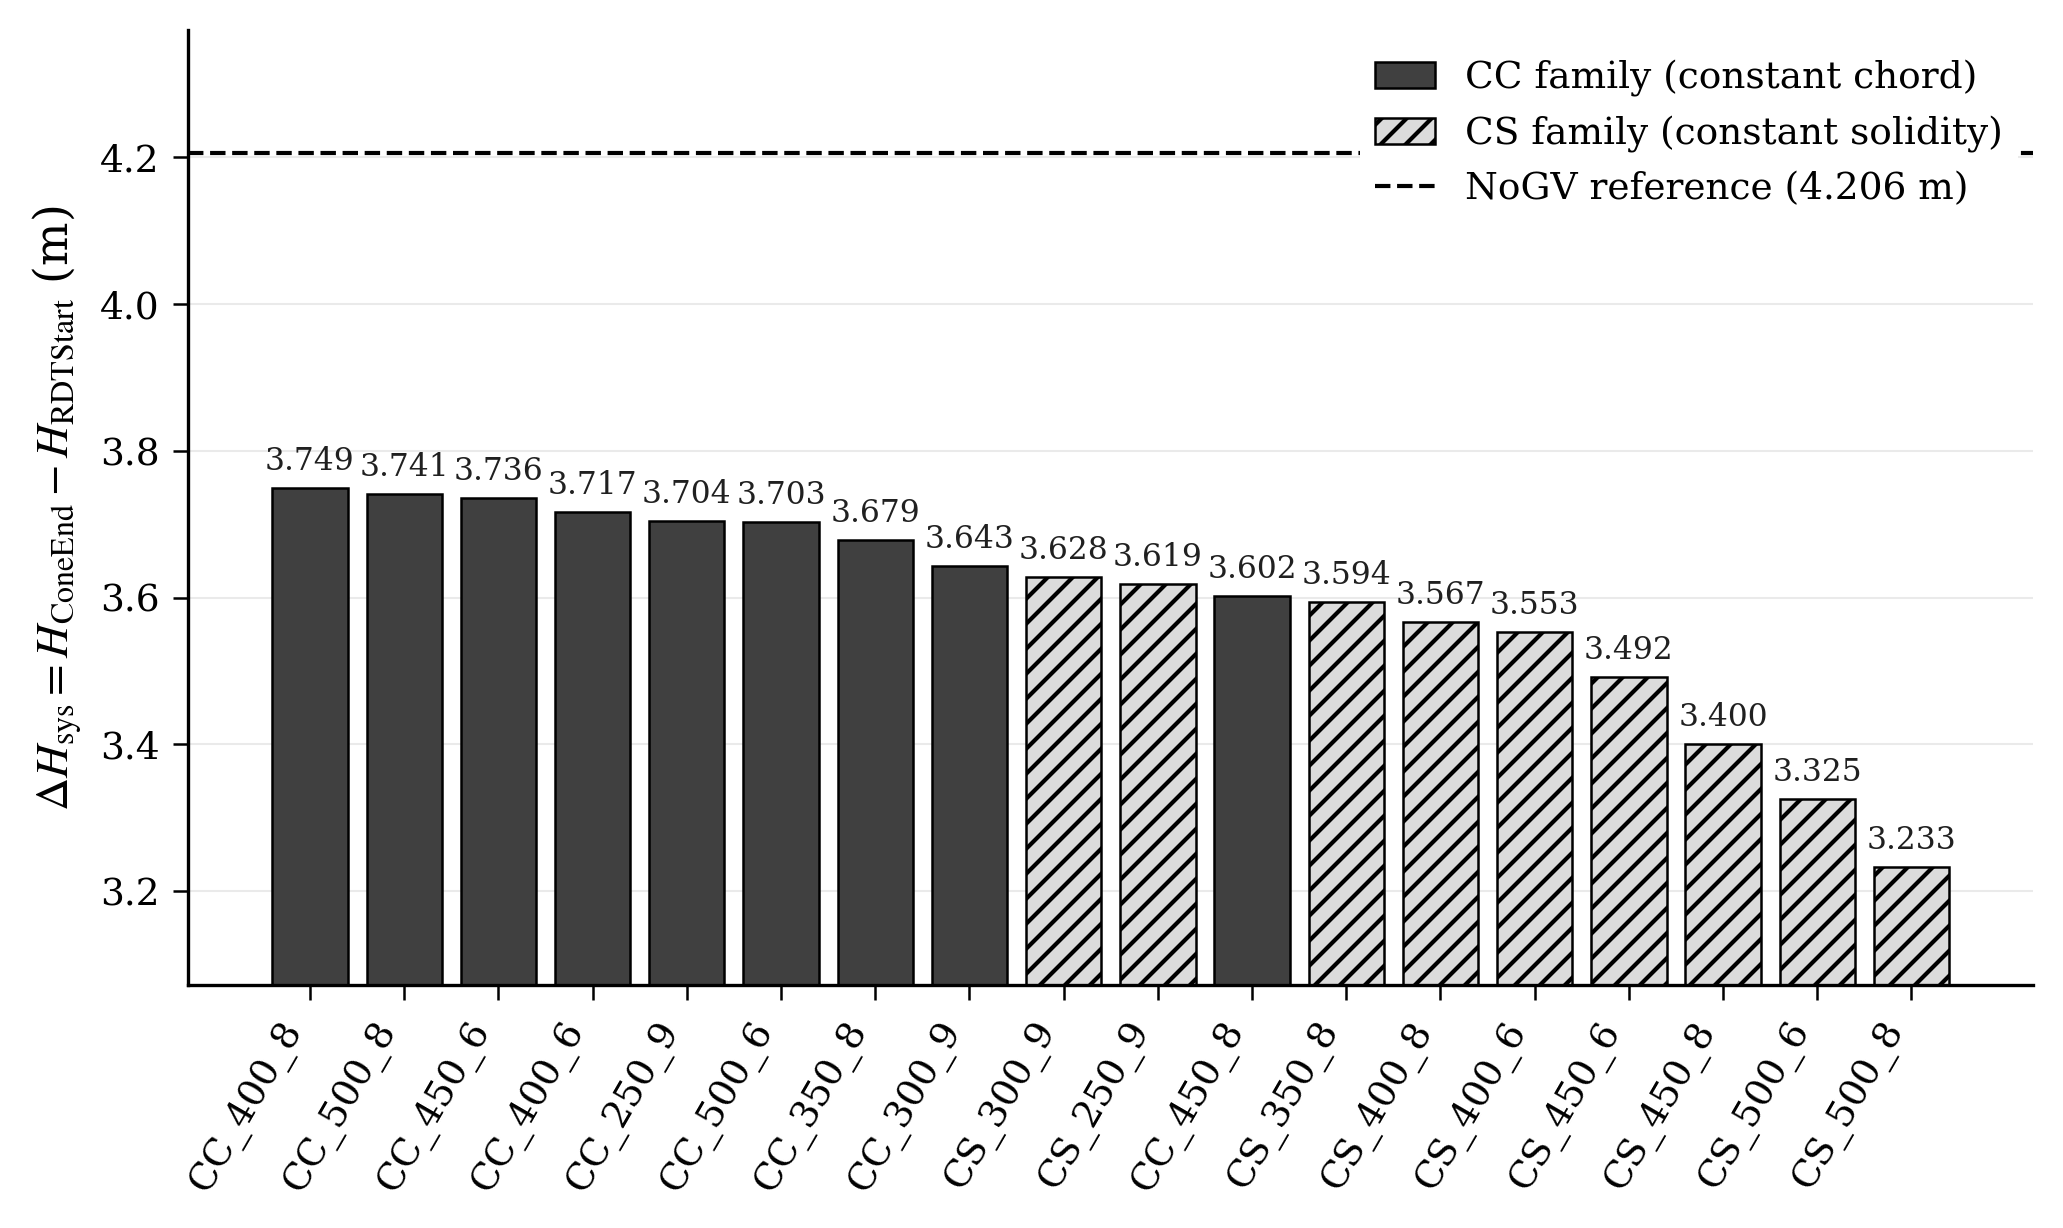
\includegraphics[width=0.95\linewidth]{Figures/Results/fig_4_3_HI_bar.png}
\caption{System head increase $\Delta H_{\mathrm{sys}} = H_{\mathrm{ConeEnd}} - H_{\mathrm{RDTStart}}$ for the $18$-case screening matrix, sorted from highest to lowest. The dashed line marks the NoGV swirl reference at $3.96$~m. CC family is shown with solid grey fill; CS family is shown with diagonal hatching. Values are read from \texttt{Results\_correctRDT.csv}.}
\label{fig:hi-bar}
\end{figure}

The highest $\Delta H_{\mathrm{sys}}$ in the GV matrix is \texttt{CC\_400\_8} at $3.75$~m, and the lowest is \texttt{CS\_500\_8} at $3.23$~m. The range across the matrix is $0.52$~m, about $16\%$ of the median.

The NoGV reference delivers higher $\Delta H_{\mathrm{sys}}$ than any GV configuration. The reference has no GV passage and therefore no associated head loss. Any guide vane inserted in the duct trades some head for swirl reduction. The screening question is the shape of that trade-off, not whether the trade-off exists.

A simple chord rule does not predict the ordering within each family. In the CC family, \texttt{CC\_400\_8} sits at the top and \texttt{CC\_450\_8} near the bottom; the highest-HI CC configuration is not the longest-chord case. In the CS family, the longest chord corresponds to the lowest HI (\texttt{CS\_500\_8}). The two families respond differently to chord length, which Section~\ref{sec:family-and-chord-trends} examines.

The family separation is sharp across the matrix. The five highest-HI configurations all belong to the CC family. The five lowest-HI configurations all belong to the CS family. The clean split motivates a family-level statistical comparison rather than case-by-case discussion.

\subsection{Head-loss decomposition}
\label{sec:hl-decomposition}

The total head loss between \texttt{GVStart} and \texttt{BendEnd} is decomposed into three sub-sections. The guide-vane passage loss $\mathrm{HL_{GV}}$ is taken between \texttt{GVStart} and the fixed axial reference plane $z = -0.680$~m (\texttt{GVEnd\_z680}), placed downstream of the longest vane trailing edge. The cone-section loss $\mathrm{HL_{cone}}$ is taken between \texttt{GVEnd\_z680} and \texttt{ConeEnd}. The bend loss $\mathrm{HL_{bend}}$ is taken between \texttt{BendStart} and \texttt{BendEnd}. The fixed $z680$ reference ensures that the GV-passage budget is comparable across configurations with different chord lengths.

Figure~\ref{fig:hl-stacked} shows the three components as a stacked bar for the $18$ configurations and the NoGV reference. Numerical values are listed in Table~\ref{tab:hl-decomposition}.

\begin{figure}[H]
\centering
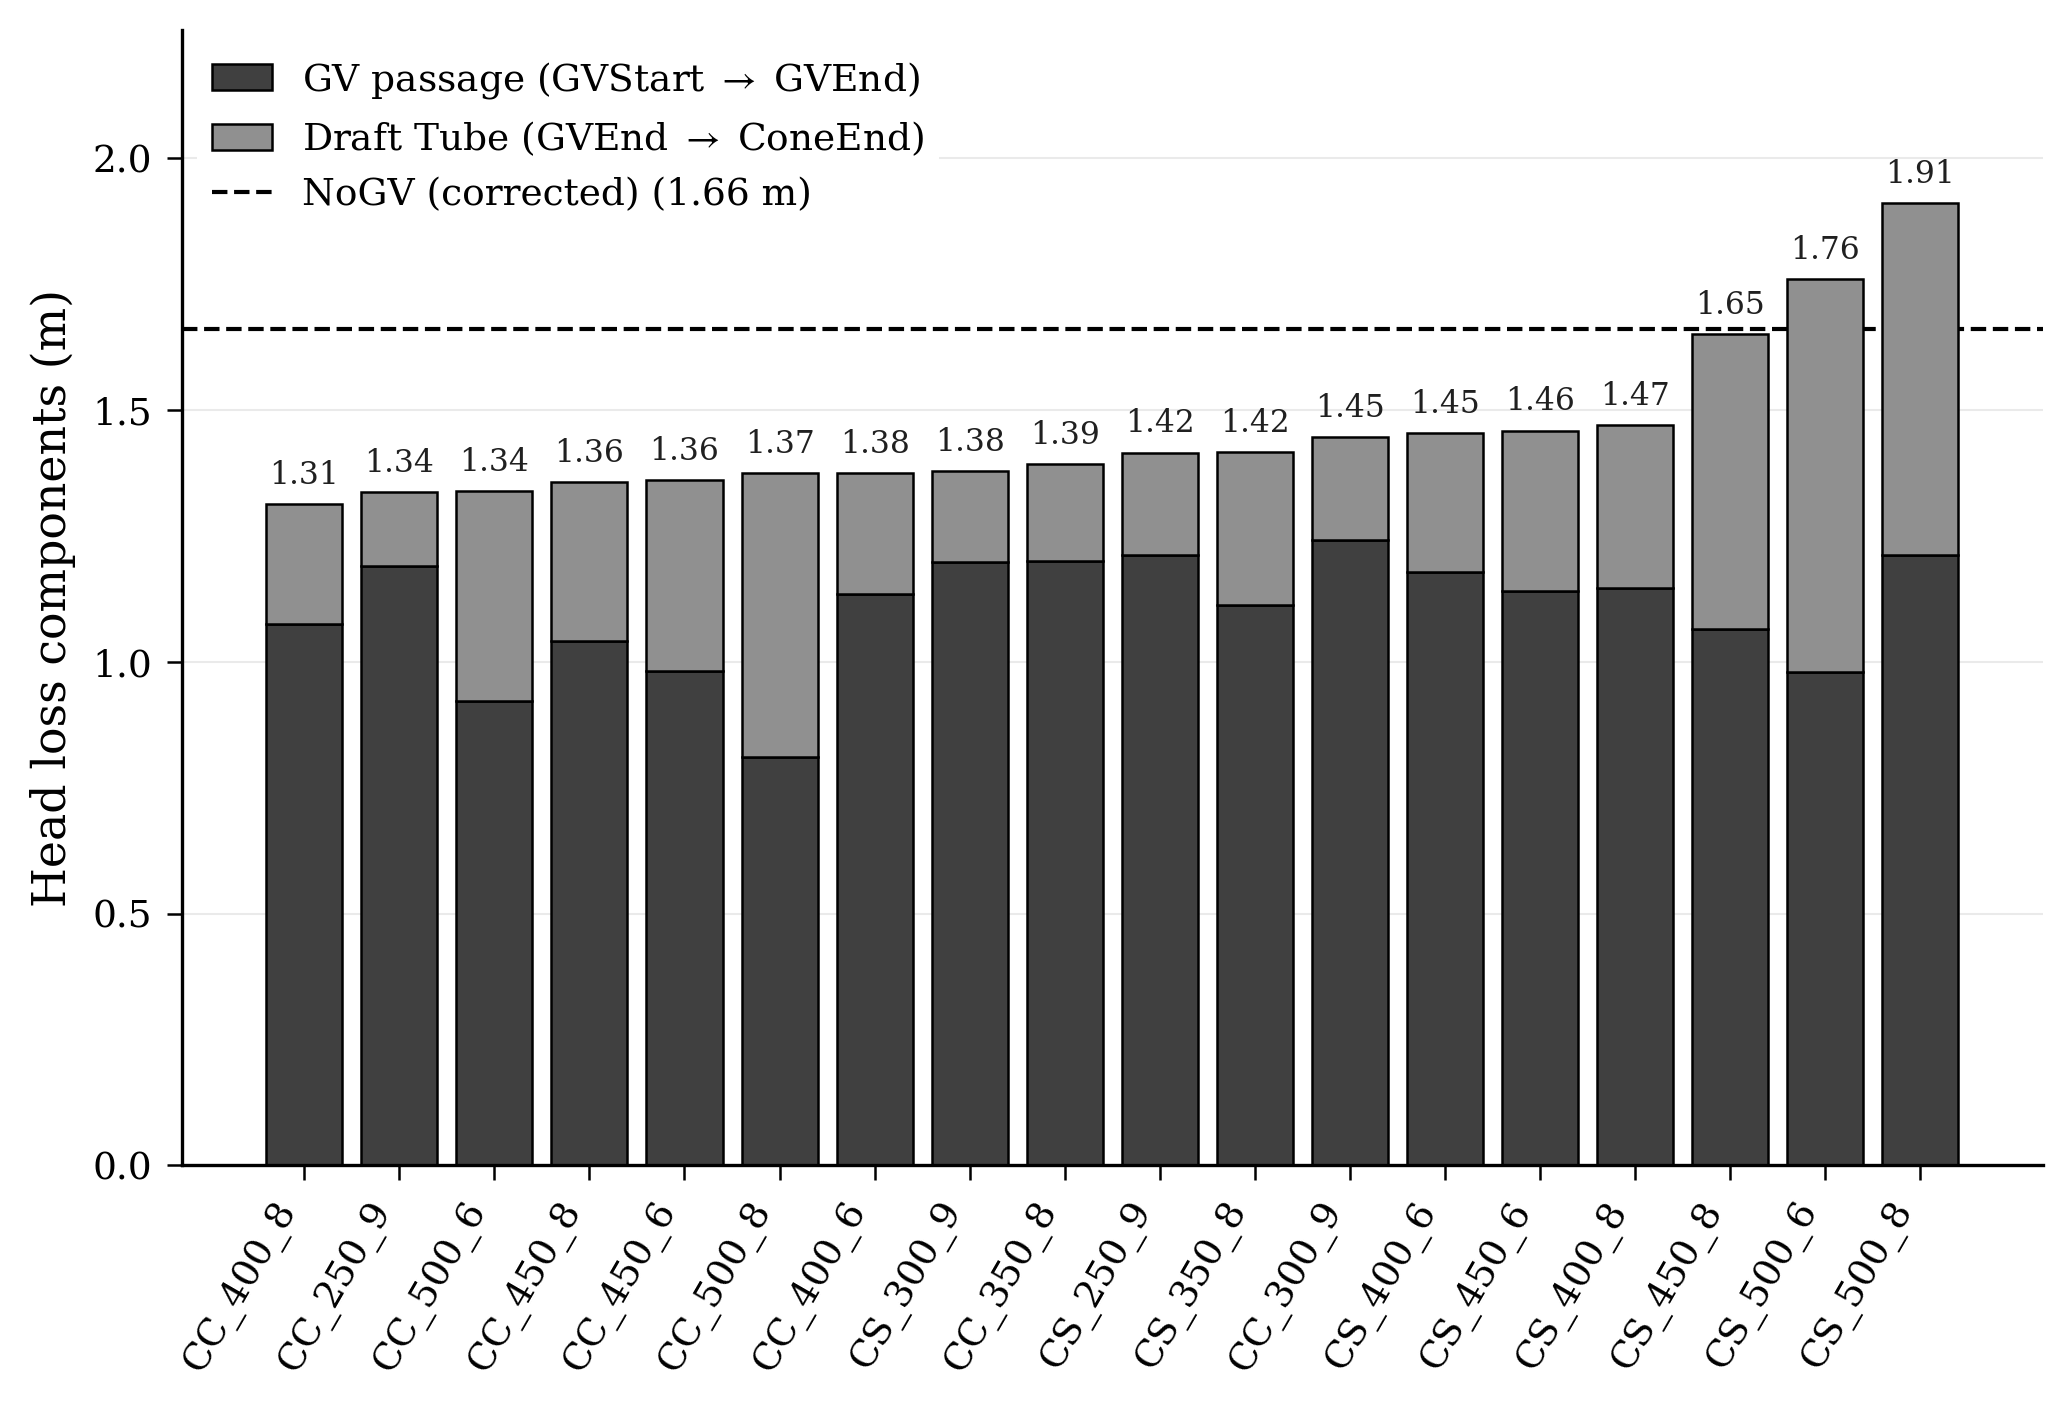
\includegraphics[width=0.95\linewidth]{Figures/Results/fig_4_4_HL_stacked_bar.png}
\caption{Head-loss decomposition into GV passage, cone section, and bend for the $18$-case screening matrix and the NoGV swirl reference. The dashed line marks the NoGV total head loss of $1.72$~m. Sub-section definitions follow Table~\ref{tab:hl-decomposition}.}
\label{fig:hl-stacked}
\end{figure}

The guide-vane passage dominates the loss budget for every GV configuration, accounting for $58\%$ to $87\%$ of the total. The cone-section loss is the second largest contributor and varies most strongly with design: from $0.146$~m (\texttt{CC\_250\_9}) to $0.779$~m (\texttt{CS\_500\_6}), a factor of more than five across the matrix. The bend loss is essentially negligible for any GV configuration, ranging from $0.014$ to $0.058$~m. The same bend section produces $0.393$~m of loss for the NoGV reference, an order of magnitude higher.

The bend collapse is the most pronounced single effect in the loss decomposition. As soon as any guide vane reduces the upstream swirl, the bend section essentially stops generating measurable head loss. The mechanism is examined in Section~\ref{sec:bend-hl-collapse}. The relevant observation for the screening interpretation is that the bend section is not where configurations differentiate. The differentiation happens in the trade-off between $\mathrm{HL_{GV}}$ and $\mathrm{HL_{cone}}$, which the family-level analysis examines next.

\begin{table}[H]
\centering
\footnotesize
\caption{Head-loss decomposition for the $18$-case screening matrix and the NoGV swirl reference. $\mathrm{HL_{GV}}$ is taken between \texttt{GVStart} and the fixed axial reference plane at $z = -0.680$~m. $\mathrm{HL_{cone}}$ is taken between this reference plane and \texttt{ConeEnd}. $\mathrm{HL_{bend}}$ is taken between \texttt{BendStart} and \texttt{BendEnd}. $\mathrm{HL_{total}}$ is the sum from \texttt{GVStart} to \texttt{BendEnd}. All values in metres. For the NoGV reference the $\mathrm{HL_{GV}}$ column reports the head loss in the same axial section without any guide vane present.}
\label{tab:hl-decomposition}
\begin{tabular}{l rrrr}
\hline
Case & $\mathrm{HL_{GV}}$ & $\mathrm{HL_{cone}}$ & $\mathrm{HL_{bend}}$ & $\mathrm{HL_{total}}$ \\ \hline
\texttt{CS\_500\_8} & $1.211$ & $0.700$ & $0.014$ & $1.910$ \\
\texttt{CS\_500\_6} & $0.980$ & $0.779$ & $0.022$ & $1.756$ \\
\texttt{CS\_450\_8} & $1.064$ & $0.586$ & $0.036$ & $1.652$ \\
\texttt{CS\_450\_6} & $1.140$ & $0.319$ & $0.022$ & $1.459$ \\
\texttt{CS\_400\_8} & $1.146$ & $0.324$ & $0.026$ & $1.464$ \\
\texttt{CS\_400\_6} & $1.179$ & $0.275$ & $0.036$ & $1.445$ \\
\texttt{CS\_350\_8} & $1.113$ & $0.303$ & $0.025$ & $1.412$ \\
\texttt{CS\_300\_9} & $1.197$ & $0.182$ & $0.029$ & $1.366$ \\
\texttt{CS\_250\_9} & $1.211$ & $0.204$ & $0.050$ & $1.414$ \\
\texttt{CC\_500\_8} & $0.811$ & $0.563$ & $0.022$ & $1.371$ \\
\texttt{CC\_500\_6} & $0.921$ & $0.418$ & $0.016$ & $1.333$ \\
\texttt{CC\_450\_8} & $1.042$ & $0.314$ & $0.016$ & $1.348$ \\
\texttt{CC\_450\_6} & $0.981$ & $0.379$ & $0.016$ & $1.352$ \\
\texttt{CC\_400\_8} & $1.074$ & $0.239$ & $0.016$ & $1.308$ \\
\texttt{CC\_400\_6} & $1.135$ & $0.240$ & $0.058$ & $1.374$ \\
\texttt{CC\_350\_8} & $1.199$ & $0.194$ & $0.021$ & $1.388$ \\
\texttt{CC\_300\_9} & $1.242$ & $0.204$ & $0.043$ & $1.428$ \\
\texttt{CC\_250\_9} & $1.191$ & $0.146$ & $0.045$ & $1.334$ \\
NoGV swirl          & $0.528$ & $1.256$ & $0.393$ & $1.723$ \\
\hline
\end{tabular}
\end{table}

\subsection{Family-level trends and chord trends}
\label{sec:family-and-chord-trends}

The CC and CS families partition the screening matrix into two groups of nine configurations each. Mean values per family are reported in Table~\ref{tab:family-means}.

\begin{table}[H]
\centering
\small
\caption{Family-mean values computed across the nine CC and nine CS configurations of the screening matrix. The angle metric $|\alpha|_{\mathrm{ConeEnd}}$ is included for context; its dependence on chord is examined in Section~\ref{sec:swirl-recovery}.}
\label{tab:family-means}
\begin{tabular}{l rr}
\hline
Quantity & CC mean & CS mean \\ \hline
$\Delta H_{\mathrm{sys}}$ (m)        & $3.70$ & $3.49$ \\
$\mathrm{HL_{GV}}$ (m)                & $1.07$ & $1.14$ \\
$\mathrm{HL_{cone}}$ (m)              & $0.30$ & $0.41$ \\
$\mathrm{HL_{bend}}$ (m)              & $0.028$ & $0.029$ \\
$\mathrm{HL_{total}}$ (m)             & $1.36$ & $1.54$ \\
$|\alpha|_{\mathrm{ConeEnd}}$ (deg)   & $23.5$ & $23.0$ \\
\hline
\end{tabular}
\end{table}

The CC family delivers higher mean $\Delta H_{\mathrm{sys}}$ ($3.70$~m) than CS ($3.49$~m), a difference of $0.21$~m or about $6\%$. The CC family also shows lower mean total head loss ($1.36$~m versus $1.54$~m). The CC advantage is not the result of a single sub-section: CC loses less in the guide-vane passage ($1.07$~m mean versus $1.14$~m) and less in the cone section ($0.30$~m versus $0.41$~m). Both contributions are separately measurable in the decomposition and they reinforce each other.

The cone-section difference is the larger of the two and explains most of the family-level HL gap ($0.11$~m of the $0.18$~m total). CS configurations leave more residual swirl after the trailing edge. The constant-solidity construction concentrates more turning capability at the outer span, where the dynamic head is highest, and the strong outer-span turning produces stronger tangential gradients at \texttt{GVEnd}. These gradients then mix through the contraction and appear in $\mathrm{HL_{cone}}$. CC achieves a comparable axial-flow rotation with less aggressive outer-span turning and pays a smaller cone-mixing penalty.

A caveat applies to the angle metric. The family-mean $|\alpha|_{\mathrm{ConeEnd}}$ is similar for the two families ($23.5^\circ$ CC versus $23.0^\circ$ CS, a difference of only $0.5^\circ$). The family-mean angle is a poor summary statistic for the screening matrix because it hides a strong interaction between family and chord length. Section~\ref{sec:swirl-recovery} examines this interaction directly. The short version is that CS responds more strongly to chord: the $|\alpha|_{\mathrm{ConeEnd}}$ spread across the CS family is $26^\circ$ from \texttt{CS\_250\_9} to \texttt{CS\_500\_8}, compared to $19^\circ$ across the CC family. At the longest chord, CS clearly outperforms CC on residual angle; at the shortest chord the two families are nearly identical.

The chord trends within each family in terms of head balance are not symmetric. Within the CC family, lengthening the chord from $250$ to $500$~mm decreases $\mathrm{HL_{GV}}$ from $1.19$ to $0.81$~m and increases $\mathrm{HL_{cone}}$ from $0.15$ to $0.56$~m. The two effects nearly cancel: total head loss changes from $1.33$ to $1.37$~m and $\Delta H_{\mathrm{sys}}$ changes from $3.70$ to $3.74$~m. Lengthening the chord shifts the loss from the GV passage to the cone section, but the head balance is robust. Within the CS family the same chord change keeps $\mathrm{HL_{GV}}$ essentially flat ($1.21$ to $1.21$~m), strongly increases $\mathrm{HL_{cone}}$ from $0.20$ to $0.70$~m, and consequently lowers $\Delta H_{\mathrm{sys}}$ from $3.62$ to $3.23$~m. Lengthening the chord in the CS family adds direct cost without a compensating reduction in GV-passage loss.

The asymmetry tells the design story for $\Delta H_{\mathrm{sys}}$: the CC family is more forgiving of chord variation in head-balance terms, while the CS family pays directly for stronger swirl recovery as the chord lengthens. The swirl-recovery side of the trade-off is examined in the next section, and the combined picture appears in the Pareto analysis in Section~\ref{sec:pareto-front}.

\section{Swirl recovery across the screening matrix}
\label{sec:swirl-recovery}

Section~\ref{sec:head-increase-and-hl} examined the head side of the trade-off. The other side is the swirl reduction each configuration achieves. Two metrics carry the analysis. The mass-averaged absolute flow angle $|\alpha|$ at \texttt{ConeEnd} is the principal RQ1 metric, since \texttt{ConeEnd} is the RPT inlet plane. The swirl number $S$, defined as the axial flux of angular momentum normalised by the axial momentum flux and a reference radius, characterises how the angular-momentum content evolves through the duct. Both metrics are reported. $|\alpha|$ is dimensionally familiar and reports the local flow direction; $S$ weights tangential velocity by radius and captures where the swirl energy is located.

\subsection{Mean flow angle at \texttt{ConeEnd}}
\label{sec:mean-flow-angle}

Table~\ref{tab:swirl-recovery-metrics} lists $|\alpha|_{\mathrm{ConeEnd}}$ together with the donut-region swirl number at \texttt{GVStart} and \texttt{GVEnd6} and the full-pipe swirl number at \texttt{ConeEnd} and \texttt{BendEnd}.

The screening matrix spans $|\alpha|_{\mathrm{ConeEnd}}$ from $9.1^\circ$ (\texttt{CS\_500\_8}) to $35.1^\circ$ (\texttt{CS\_250\_9}). The factor of nearly four between best and worst is the largest relative spread of any screening metric. Both extremes are in the same family. The CS construction is the most powerful when chord is long and the least effective when chord is short.

Long chord wins in both families. The three best configurations are \texttt{CS\_500\_8} ($9.1^\circ$), \texttt{CS\_500\_6} ($13.1^\circ$), and \texttt{CC\_500\_8} ($16.5^\circ$). The worst pair pairs near-identical angles from short-chord, high-vane-count cases: \texttt{CS\_250\_9} at $35.1^\circ$ and \texttt{CC\_250\_9} at $35.0^\circ$. The chord effect is not symmetric across families. Going from $250$ to $500$~mm drops the residual angle by $26^\circ$ in CS but only $19^\circ$ in CC. The CS family construction concentrates more turning at the outer span, where the dynamic head is highest. When the chord is long enough, that outer-span turning removes more angular momentum than the equivalent CC design and the family pulls ahead. When the chord is short, the CS family loses this advantage and the two families converge.

The four corners of the design space organise the picture cleanly. Long chord with CS gives the lowest angle. Long chord with CC gives moderate angle and the highest $\Delta H_{\mathrm{sys}}$. Short chord with CS gives the worst angle. Short chord with CC gives near-equal angle to its CS counterpart at less head cost. Intermediate cases fall along smooth interpolations between these corners.

The mesh-bias caveat from Section~\ref{sec:rdt-mesh-overlap-impact} applies. Within-family rankings between adjacent chord steps (\texttt{CC\_450\_6} versus \texttt{CC\_400\_8}, for example) are not anchor-confirmed. Family-level and corner-of-matrix comparisons are robust across both setups.

\begin{table}[H]
\centering
\footnotesize
\caption{Swirl-recovery metrics for the $18$-case screening matrix and the NoGV swirl reference. $|\alpha|_{\mathrm{ConeEnd}}$ is the mass-averaged absolute flow angle at the RPT inlet plane. $S_{\mathrm{GVStart}}$ and $S_{\mathrm{GVEnd6}}$ are donut-region swirl numbers (annular section between hub and shroud). $S_{\mathrm{ConeEnd}}$ and $S_{\mathrm{BendEnd}}$ are signed full-pipe swirl numbers: positive values indicate rotation in the same sense as the upstream RDT swirl, negative values indicate over-correction by the guide vanes.}
\label{tab:swirl-recovery-metrics}
\begin{tabular}{l r rrrr}
\hline
Case & $|\alpha|_{\mathrm{ConeEnd}}$ (deg) & $S_{\mathrm{GVStart}}$ & $S_{\mathrm{GVEnd6}}$ & $S_{\mathrm{ConeEnd}}$ & $S_{\mathrm{BendEnd}}$ \\ \hline
\texttt{CS\_500\_8} & $9.1$  & $1.22$ & $0.15$ & $+0.17$ & $-0.11$ \\
\texttt{CS\_500\_6} & $13.1$ & $1.24$ & $0.20$ & $+0.29$ & $-0.02$ \\
\texttt{CS\_450\_8} & $16.7$ & $1.12$ & $0.37$ & $+0.22$ & $-0.23$ \\
\texttt{CS\_450\_6} & $22.3$ & $1.01$ & $0.55$ & $-0.30$ & $-0.75$ \\
\texttt{CS\_400\_8} & $22.2$ & $0.94$ & $0.52$ & $-0.23$ & $-0.78$ \\
\texttt{CS\_400\_6} & $29.3$ & $0.94$ & $0.63$ & $-0.20$ & $-1.16$ \\
\texttt{CS\_350\_8} & $28.1$ & $0.93$ & $0.65$ & $-0.45$ & $-1.43$ \\
\texttt{CS\_300\_9} & $30.7$ & $0.90$ & $0.77$ & $-0.72$ & $-1.94$ \\
\texttt{CS\_250\_9} & $35.1$ & $0.87$ & $0.94$ & $-1.15$ & $-2.31$ \\
\texttt{CC\_500\_8} & $16.5$ & $0.96$ & $0.31$ & $+0.13$ & $-0.23$ \\
\texttt{CC\_500\_6} & $17.3$ & $0.91$ & $0.38$ & $+0.11$ & $-0.24$ \\
\texttt{CC\_450\_8} & $20.6$ & $0.84$ & $0.47$ & $-0.08$ & $-0.43$ \\
\texttt{CC\_450\_6} & $25.5$ & $0.85$ & $0.59$ & $-0.24$ & $-0.89$ \\
\texttt{CC\_400\_8} & $21.5$ & $0.88$ & $0.51$ & $-0.26$ & $-0.74$ \\
\texttt{CC\_400\_6} & $28.2$ & $0.88$ & $0.74$ & $-0.86$ & $-1.04$ \\
\texttt{CC\_350\_8} & $25.1$ & $0.87$ & $0.60$ & $-0.39$ & $-1.09$ \\
\texttt{CC\_300\_9} & $21.4$ & $0.86$ & $0.69$ & $-0.42$ & $-1.32$ \\
\texttt{CC\_250\_9} & $35.0$ & $0.82$ & $0.88$ & $-1.05$ & $-1.96$ \\
NoGV swirl          & $53.6$ & $1.83$ & $2.18$ & $-0.92$ & $-6.62$ \\
\hline
\end{tabular}
\end{table}

\subsection{Swirl number evolution through the duct}
\label{sec:swirl-number-evolution}

The angle metric reports a local quantity at one plane. The swirl number tracks angular-momentum flux through the duct and reveals how each configuration redistributes the tangential momentum left over from the guide vane.

At \texttt{GVStart}, the donut-region swirl number ranges from $0.82$ (\texttt{CC\_250\_9}) to $1.24$ (\texttt{CS\_500\_6}) across the GV matrix. The NoGV reference shows $S_{\mathrm{GVStart}} = 1.83$, well above any GV case. The presence of the vanes alters the upstream swirl even at the leading edge plane through subsonic upstream feedback of the GV blockage on the RDT wake. The effect is small in absolute terms but consistent: longer-chord and lower-vane-count configurations push their influence slightly further upstream.

At the deepest GVEnd plane (\texttt{GVEnd6}), $S$ collapses by a factor of two to eight relative to \texttt{GVStart}. \texttt{CS\_500\_8} drops from $1.22$ to $0.15$, an eight-fold reduction. \texttt{CC\_250\_9} drops only from $0.82$ to $0.88$, essentially unchanged, because the short chord and high vane count produce a vane stack that under-turns and leaves the donut-region swirl close to its incoming value. The contrast between these two extremes is the screening result in one comparison.

Between \texttt{GVEnd6} and \texttt{ConeEnd} the flow transitions from the annular GV region to the full pipe cross-section and undergoes contraction. The swirl number computed on the two planes is not directly comparable in magnitude, since the reference radius and area change. The sign is comparable, and the sign change between \texttt{GVEnd6} and \texttt{ConeEnd} carries information about the GV over-correction examined in the next subsection.

The bend amplifies what enters it. For low-recovery configurations such as \texttt{CC\_250\_9} and \texttt{CS\_250\_9}, the absolute swirl number at \texttt{BendEnd} roughly doubles relative to \texttt{ConeEnd} in magnitude. The same comparison for the Pareto candidates shows almost no change: \texttt{CS\_500\_8} has $|S|$ of $0.17$ at \texttt{ConeEnd} and $0.11$ at \texttt{BendEnd}. The detailed mechanism appears in Section~\ref{sec:bend-hl-collapse}; the screening conclusion is that the bend penalises configurations with weak swirl recovery far more than it penalises strong-recovery configurations.

\subsection{Sign of residual swirl and pump-mode pre-rotation implications}
\label{sec:sign-of-swirl}

Sign matters here. The sign convention for $S$ at \texttt{ConeEnd} reflects the rotation direction relative to the upstream RDT swirl. A positive value means the residual swirl rotates in the same sense as the original RDT swirl: the guide vanes have under-corrected the flow. A negative value means the residual swirl rotates against the original direction: the vanes have over-corrected the flow, producing what the downstream RPT experiences as counter-rotation, or negative pre-rotation (NPR).

The split across the matrix is uneven. Only five configurations show positive $S_{\mathrm{ConeEnd}}$: \texttt{CS\_500\_8} ($+0.17$), \texttt{CS\_500\_6} ($+0.29$), \texttt{CS\_450\_8} ($+0.22$), \texttt{CC\_500\_8} ($+0.13$), and \texttt{CC\_500\_6} ($+0.11$). The remaining thirteen configurations over-correct and present NPR to the downstream RPT. The over-correction magnitude grows with shorter chord: \texttt{CC\_250\_9} reaches $S_{\mathrm{ConeEnd}} = -1.05$, a substantial NPR magnitude.

The implication for downstream RPT operation is non-trivial. The pump-mode cavitation study of Jenssen~\cite{Jenssen2020} on the same RPT geometry showed that NPR is qualitatively favourable for cavitation behaviour at high-flow operating points. The required cavitation number $\sigma_{\mathrm{req}}$ decreased by up to $25\%$ with imposed NPR, while PPR increased it by up to $93\%$. The five PPR configurations in the present matrix are therefore not unambiguously the best for the full RDT--GV--RPT system, even though they sit closest to zero residual swirl on the angle metric. A moderate-magnitude NPR design may be preferable for cavitation, provided the angle magnitude stays below the threshold where pump efficiency degrades sharply.

Jenssen also observed that any pre-rotation reduced pump efficiency relative to the no-pre-rotation case. The optimal residual swirl from a full-system perspective is therefore neither zero nor arbitrarily large in either direction. It is a finite NPR magnitude small enough to keep the efficiency penalty acceptable and large enough to gain the cavitation benefit. The present screening matrix can identify candidate configurations in this band but cannot quantify the trade-off without coupled GV--RPT simulations, which fall outside the scope of this thesis and appear as future work in Chapter~\ref{chap:future_work}.

The screening conclusion on sign is that the Pareto-front evaluation in Section~\ref{sec:pareto-front} does not penalise NPR cases for not being closer to zero. The angle magnitude $|\alpha|_{\mathrm{ConeEnd}}$ remains the primary metric. The sign carries additional information that the final candidate selection in Section~\ref{sec:synthesis} weighs explicitly.

\section{FFT analysis of the transient RDT-GV simulations}
\label{sec:results-fft}
 
Two transient RDT-GV simulations were run at $n = 650$~rpm to test the Tyler-Sofrin prediction in the present geometry. The two cases are diagnostic blade-count configurations; the final hydraulic candidate is selected separately from the steady screening matrix. \texttt{CC\_450\_7} is the project-work baseline ($Z_r = Z_s = 7$, $m_{\min} = 0$); the Tyler-Sofrin analysis predicts a synchronous breathing mode at $f_{\mathrm{BPF}}$. \texttt{CC\_400\_6} is the spinning-mode comparator ($Z_s = 6$, $m_{\min} = 1$) drawn from the screening matrix. Both runs were initialised from the same baseline restart at $t = 2.447$~s and continued for 15 rotor revolutions to $t = 3.831$~s.
\subsection{Peak amplitudes at the characteristic frequencies}
\label{sec:results-peaks}
 
The FFT uses the last $N_{\mathrm{rev}} = 5$ rotor revolutions ($N = 1800$, $\Delta f = 2.167$~Hz) with a Hanning window, following the methodology in Section~\ref{sec:spec}. Time histories, the phase-folded comparison and the window-robustness check are in Appendix~\ref{app:individual_spectra} (Sections A.1-A.2).
 
Peak amplitudes at $f_n$ and $f_{\mathrm{BPF}}$ are listed in Tables~\ref{tab:peak_amplitudes_450_7} and~\ref{tab:peak_amplitudes_400_6}. The ratio $A(f_{\mathrm{BPF}})/A(f_n)$ indicates whether each signal is dominated by blade-passing content or by rotor-frequency content.

\begin{table}[H]
\centering
\small
\caption{Configuration \texttt{CC\_450\_7} ($Z_r = Z_s = 7$, $c = 450$~mm). Peak amplitudes at $f_n = 10.83$~Hz and $f_{\mathrm{BPF}} = 75.83$~Hz. Wall-pressure probes are at $r/R = 0.744$. Symbols are defined in Table~\ref{tab:monitor-index}.}
\label{tab:peak_amplitudes_450_7}
\begin{tabular}{lcccc}
\hline
Signal & Unit & $A(f_n)$ & $A(f_{\mathrm{BPF}})$ & Ratio \\ \hline
$F_{\mathrm{res}}$  & N    & 5.21  & 0.56  & 0.11 \\
$M_{\mathrm{RDT}}$  & N\,m & 0.43  & 0.064 & 0.15 \\
$P_{\mathrm{in}}$   & Pa   & 71.3  & 21.9  & 0.31 \\
$P_{\mathrm{out}}$  & Pa   & 138   & 19.6  & 0.14 \\
$P_0$               & Pa   & 625   & 80.6  & 0.13 \\
$P_3$               & Pa   & 608   & 32.8  & 0.05 \\
$P_5$               & Pa   & 431   & 20.0  & 0.05 \\ \hline
\end{tabular}
\end{table}

\begin{table}[H]
\centering
\small
\caption{Configuration \texttt{CC\_400\_6} ($Z_s = 6$, $c = 400$~mm). Peak amplitudes at $f_n = 10.83$~Hz and $f_{\mathrm{BPF}} = 75.83$~Hz.}
\label{tab:peak_amplitudes_400_6}
\begin{tabular}{lcccc}
\hline
Signal & Unit & $A(f_n)$ & $A(f_{\mathrm{BPF}})$ & Ratio \\ \hline
$F_{\mathrm{res}}$  & N    & 2.96  & 1.71  & 0.58 \\
$M_{\mathrm{RDT}}$  & N\,m & 0.25  & 0.20  & 0.79 \\
$P_{\mathrm{in}}$   & Pa   & 87.7  & 28.1  & 0.32 \\
$P_{\mathrm{out}}$  & Pa   & 110   & 33.9  & 0.31 \\
$P_0$               & Pa   & 329   & 192   & 0.58 \\
$P_3$               & Pa   & 831   & 24.5  & 0.03 \\
$P_5$               & Pa   & 311   & 30.8  & 0.10 \\ \hline
\end{tabular}
\end{table}

A spectral comparison of the two configurations for the four most informative signals is shown in Figure~\ref{fig:compare_spectra}.

\begin{figure}[H]
\centering
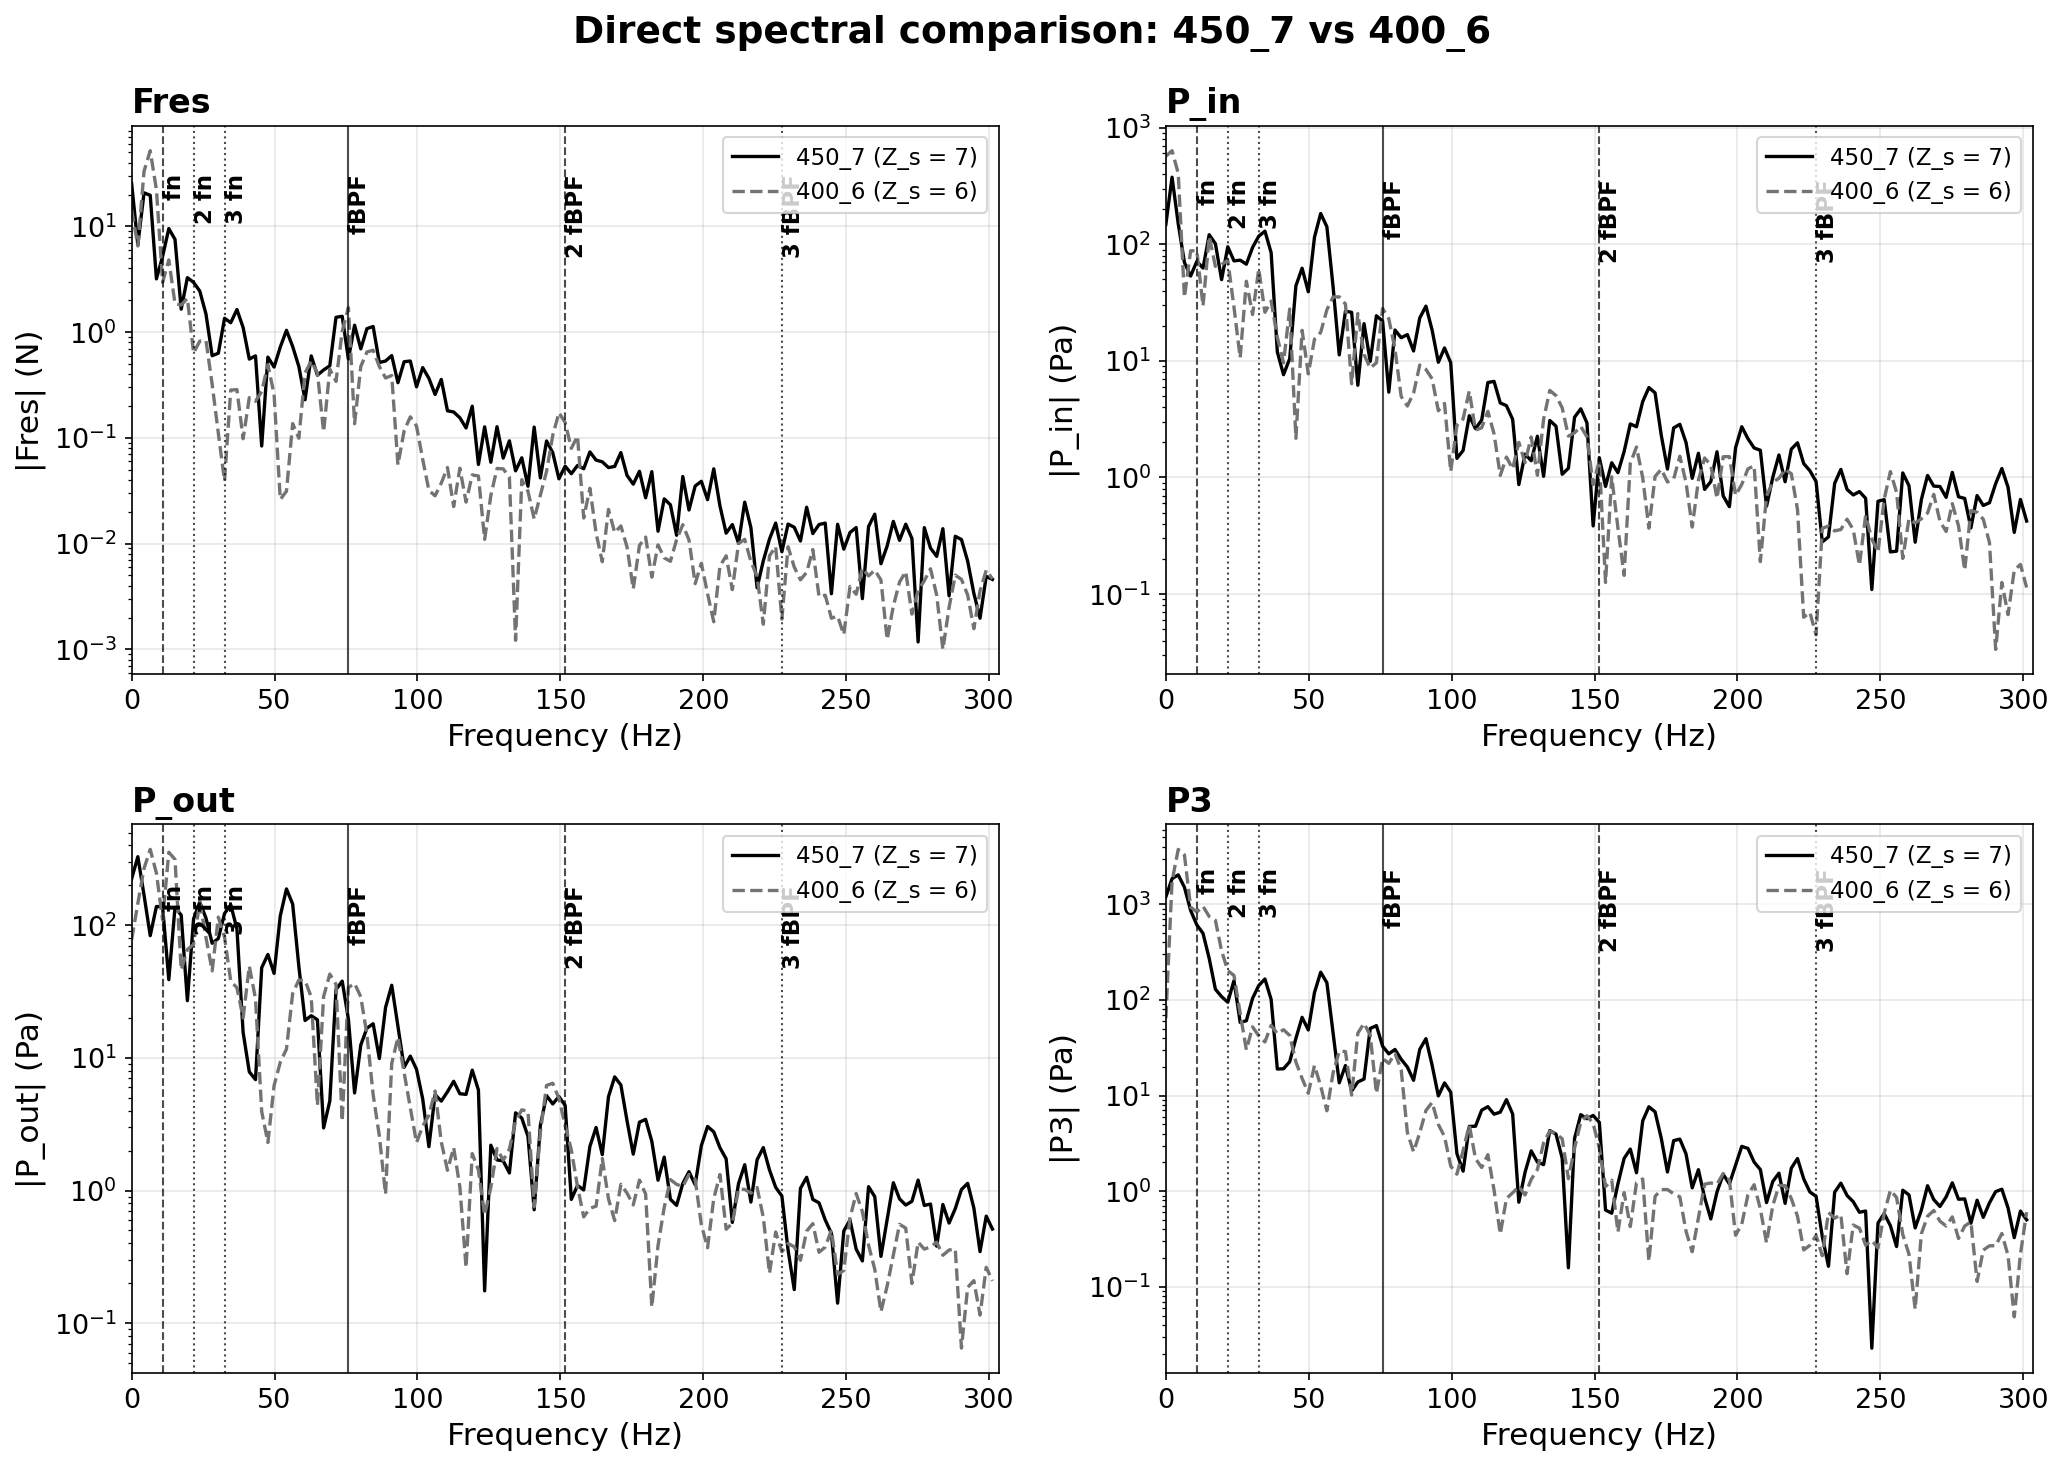
\includegraphics[width=0.99\linewidth]{Figures/FFT/comparison/compare_spectra_450_7_vs_400_6.png}
\caption{Spectral comparison of \texttt{CC\_450\_7} (solid red) and \texttt{CC\_400\_6} (dashed blue) for $F_{\mathrm{res}}$, $P_{\mathrm{in}}$, $P_{\mathrm{out}}$ and $P_3$. Vertical lines mark $f_n$ and harmonics (red) and $f_{\mathrm{BPF}}$ and harmonics (black).}
\label{fig:compare_spectra}
\end{figure}

The bar-chart amplitude comparison and the per-signal $f_n$-vs-$f_{\mathrm{BPF}}$ plots are in Appendix~\ref{app:individual_spectra} (Section A.3). Three observations stand out.

\paragraph{Observation 1: blade-passing forcing is weak.}
The cyclic force amplitude at $f_{\mathrm{BPF}}$ is $0.56$~N for \texttt{CC\_450\_7} and $1.71$~N for \texttt{CC\_400\_6}, corresponding to $0.07\,\%$ and $0.27\,\%$ of the mean vane loads. Both values are below the $0.5\,\%$ diagnostic threshold of~\cite{Egusquiza2006}. Low-frequency content dominates the unsteady vane loading; deterministic blade-passing forcing is below the diagnostic threshold.

\paragraph{Observation 2: pressure pulsations are well below the RSI threshold.}
The normalised pulsation at the RDT-GV interface is
\begin{equation}
    \tilde{p}_{E}
    = \frac{A_p(f_{\mathrm{BPF}})}{\rho g H}
    \approx 0.04\text{-}0.06\,\%,
    \label{eq:normalised-pulsation}
\end{equation}
more than one order of magnitude below the $1\,\%$ threshold of~\cite{Brekke2015,Brekke2010} for significant rotor-stator interaction.

\paragraph{Observation 3: the equal blade-count case does not show a stronger breathing-mode signature.}
\texttt{CC\_400\_6} ($m_{\min} = 1$) shows higher relative blade-passing content than \texttt{CC\_450\_7} ($m_{\min} = 0$): the ratio $A(f_{\mathrm{BPF}})/A(f_n)$ for $F_{\mathrm{res}}$ is $0.58$ in \texttt{CC\_400\_6} and $0.11$ in \texttt{CC\_450\_7}. This is not the behaviour expected from the compact-stage Tyler-Sofrin argument, where the equal blade-count case is the main concern. The absolute amplitudes remain low in both cases, and the expected coherent breathing-mode signature is weak in the present geometry. A physical interpretation is given in Section~\ref{sec:results-fft-physicalexpl}.

\subsection{Physical interpretation: large axial gap and non-uniform inflow}
\label{sec:results-fft-physicalexpl}

The absent breathing-mode signature is consistent with the large axial spacing documented in Section~\ref{sec:methods_axial_spacing}. The relevant compact-stage parameter is the rotor-stator spacing normalised by the RDT rotor chord, $a/L$, not by the duct diameter. Using the RDT chord at midspan, $L_{\mathrm{mid}} = 138.5$~mm, gives $a/L_{\mathrm{mid}} = 0.192/0.139 = 1.39$. This is about $9$ times the upper limit of the compact axial-pump guideline $a/L = 0.05$-$0.15$. The potential-interaction component of the rotor-stator pulsation is therefore strongly attenuated before the flow reaches the guide-vane row. The wake can mix and redistribute before reaching the vanes, which weakens the coherent $m = 0$ build-up predicted for a compact rotor-stator stage.

The velocity contour in Figure~\ref{fig:vel_contour_400_6} supports this interpretation. The flow is non-uniform between adjacent vane passages and shows regions of reduced velocity, consistent with recirculation in the annular space between the rim and the duct wall. The guide vanes are exposed to a mixed and asymmetric RDT wake rather than a clean $Z_r$-periodic rotor wake. A non-periodic inflow reduces the coherent build-up of the $m = 0$ component predicted by the Tyler-Sofrin framework, even when $Z_r = Z_s$.

\begin{figure}[H]
\centering
\fbox{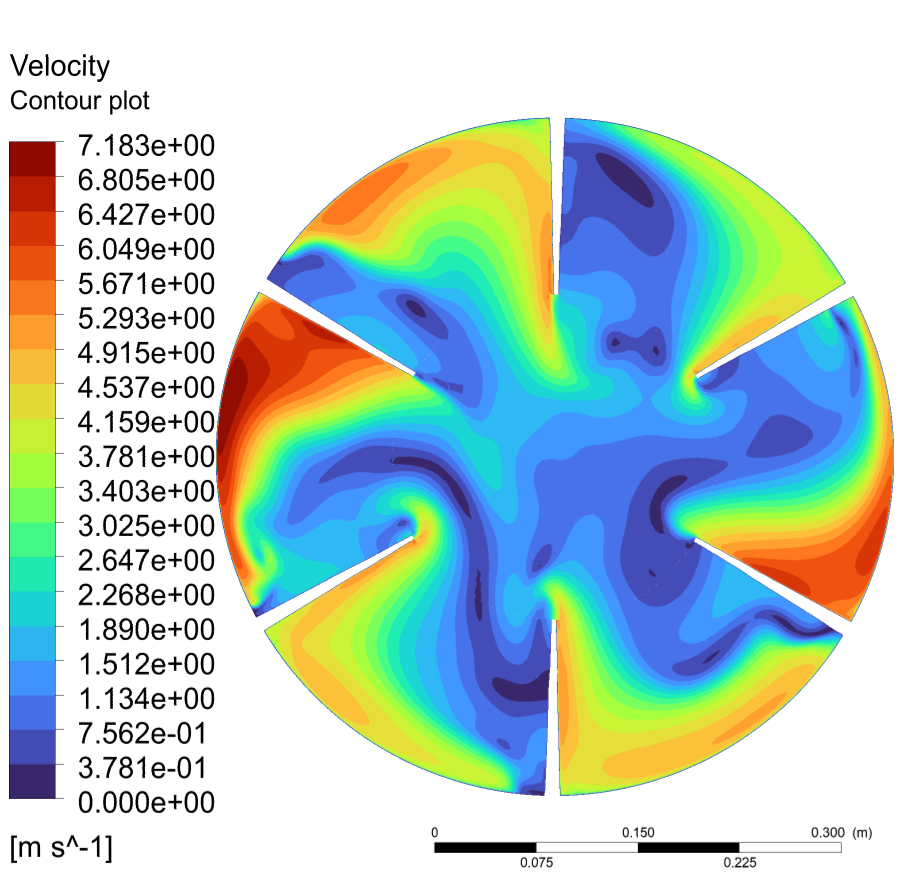
\includegraphics[width=0.55\linewidth]{Figures/FFT/CFD/vel_plot_CC_400_6_z048.png}}
\caption{Velocity magnitude contour at $z = 0.48$~m for configuration \texttt{CC\_400\_6}. The plane is located right before the Trailing edge of the GVs.}
\label{fig:vel_contour_400_6}
\end{figure}

This interpretation matches the dominant sub-rotor-frequency content in the monitor signals. Low-frequency fluctuations are the signature of slowly evolving recirculation, not deterministic blade-passing interaction.

The same mechanism explains the higher relative blade-passing content in the single-vane force signal of \texttt{CC\_400\_6}. With non-uniform inflow, the synchronous $m=0$ build-up predicted by Tyler-Sofrin for $Z_r = Z_s = 7$ does not form coherently in \texttt{CC\_450\_7}; the vanes are loaded by an asymmetric wake field. In \texttt{CC\_400\_6}, the wake-vane mismatch ($Z_r = 7$, $Z_s = 6$) produces stronger local wake-vane interaction on a single vane while the ring-integrated coherent mode remains weak. The plane-averaged pressure signals support this. The $m=0$ component is of the same order in the two cases ($21.9$~Pa versus $28.1$~Pa at the inlet plane). The higher single-vane $f_{\mathrm{BPF}}$ content in \texttt{CC\_400\_6} reflects local wake-vane interaction, not a stronger coherent ring mode.

\subsection{Implications for blade-count selection}
\label{sec:results-fft-implications}

The transient analysis establishes two results. The unsteady loading produced by the RDT-GV setup is below industrial concern thresholds for both configurations at the nominal operating point. No clear resonance signature is present in either case. The low coherent ring loading is interpreted as a consequence of the large axial gap and the asymmetric inflow rather than as proof that the equal blade-count configuration is generally safe.

The final guide-vane design is selected from the screening subset with $Z_s \neq Z_r$. The choice is conservative. The classical guideline~\cite{Brekke2015,Brekke2010,Tanaka2011,Nduwayezu2021} recommends avoiding equal rotor and stator counts when possible, especially when acoustic or structural resonance may interact with the spatial mode order. The transient runs do not indicate critical pulsation levels, but a full structural or acoustic assessment is still needed. The choice between the available options $Z_s \in \{6, 8, 9\}$ is therefore made on the basis of the hydraulic metrics presented in the next section. No modal analysis of the guide vane has been performed in this thesis. The fatigue-margin conclusion holds only if the lowest wet natural frequency is well separated from $f_{\mathrm{BPF}} = 75.83$~Hz. A finite-element modal analysis including added-mass effects is therefore recommended in Chapter~\ref{chap:future_work}.

\clearpage % Keep this at the end of the chapter

